\documentclass[11pt,letterpaper]{article}
\usepackage[T1]{fontenc}
\usepackage[utf8]{inputenc}
\usepackage{amsmath,amsthm}
\usepackage{newpxtext,newpxmath}
\usepackage[margin=0.88in,headheight=15pt]{geometry}
\usepackage{microtype,booktabs,longtable,array,tabularx}
\usepackage{xcolor,graphicx,listings,enumitem,fancyhdr,xurl,needspace}
\usepackage[most]{tcolorbox}
\usepackage[colorlinks=true,linkcolor=blue!45!black,citecolor=blue!45!black,urlcolor=blue!45!black]{hyperref}
\hypersetup{pdftitle={Asymptotic 1.8.0: Technical Review and Wolfram Language Comparison},pdfauthor={Technical review prepared for Vladimir Reshetnikov}}
\definecolor{ink}{HTML}{263A41}
\definecolor{papergray}{HTML}{F2F4F3}
\definecolor{rulegray}{HTML}{CCD4D2}
\lstdefinestyle{code}{basicstyle=\ttfamily\small,breaklines=true,columns=fullflexible,keepspaces=true,showstringspaces=false,frame=single,rulecolor=\color{rulegray},backgroundcolor=\color{papergray},xleftmargin=3pt,xrightmargin=3pt,aboveskip=9pt,belowskip=9pt}
\lstset{style=code}
\setlist{nosep,leftmargin=1.6em}
\setlength{\parskip}{5pt plus 1pt}
\setlength{\parindent}{0pt}
\setlength{\emergencystretch}{3em}
\pagestyle{fancy}\fancyhf{}
\fancyhead[L]{\small\textsc{Asymptotic 1.8.0 / Technical review}}
\fancyhead[R]{\small 9 September 2026}
\fancyfoot[C]{\thepage}
\newcommand{\code}[1]{\texttt{\small\detokenize{#1}}}
\newcommand{\OO}{\mathcal O}
\newcommand{\M}{\mathcal M}
\newcommand{\val}{\operatorname{val}}
\newcommand{\degL}{\operatorname{deg}_{L}}
\newcommand{\commit}{\texttt{07a9781212beb2eeb9ff16aa625b50ac27974078}}
\newcommand{\finding}[3]{\Needspace{8\baselineskip}\subsection{#1: #2}\noindent\textbf{Classification:} #3.\par}
\newtcolorbox{notebox}{colback=papergray,colframe=rulegray,boxrule=0.5pt,arc=1mm,left=9pt,right=9pt,top=7pt,bottom=7pt,breakable}
\newtheorem{proposition}{Proposition}[section]
\newtheorem{lemma}[proposition]{Lemma}
\newtheorem{corollary}[proposition]{Corollary}
\begin{document}
\begin{titlepage}
\vspace*{0.55in}
{\Large\color{ink}\textsc{Repository audit / Mathematical software}}\par
\vspace{0.3in}
{\Huge\bfseries Asymptotic 1.8.0}\par
\vspace{0.15in}
{\LARGE Technical review and comparison\par with Wolfram Language}\par
\vspace{0.4in}
{\large Correctness, error calculus, inverse algorithms,\par interoperability, performance, and development priorities}\par
\vspace{0.55in}
\begin{tabular}{@{}ll}
Prepared for & Vladimir Reshetnikov\\[5pt]
Repository & \url{https://github.com/VladimirReshetnikov/Asymptotic}\\[5pt]
Reviewed version & 1.8.0\\[5pt]
Commit & \commit\\[5pt]
Commit timestamp & 9 September 2026, 19:01:30 UTC\\[5pt]
Review date & 9 September 2026
\end{tabular}
\vfill
\begin{notebox}
\textbf{Evidence boundary.} This is a source-level technical audit with independently executed mathematical checks. The Wolfram connector failed to connect; no native Wolfram package execution or new Wolfram timing measurement was obtained. Source-traced behavior is identified as such. The archive contains native regression candidates and a comparison runner to complete that validation on a local installation.
\end{notebox}
\end{titlepage}

\section*{Executive assessment}
\addcontentsline{toc}{section}{Executive assessment}
The repository has grown into a substantial real-asymptotic computation system, not just an alternative implementation of \code{InverseSeries}. Its strongest contribution is the combination of sparse exact-weight inversion, complete logarithmic coefficient blocks, explicit one-sided coordinates, transported remainder information, and several specialized inverse scales. Gamma and Barnes inverses retain an exact Lambert core rather than flattening a useful hierarchy prematurely. The native special-function importer, in contrast, intentionally delegates coefficient generation to Wolfram's \code{Series} and adds real-domain validation and an error-transport layer. These are complementary roles, not a reason to describe all special-function support as independently implemented.\cite{repo-guide,repo-core,repo-gamma,repo-native}

The principal release risk is not a lack of features. It is the integrity of the precision contract across operations and representation changes. The audit identifies a concrete nonlinear-boundary error, a real-branch gap for fractional powers of pure remainders, a lossy native-series export, and an allocation path that can turn a two-term sparse expression into an enormous dense vector. It also identifies a refinement-demand failure, avoidable multi-index enumeration on supposedly grouped/Newton paths, and an unnecessarily restrictive treatment of commensurate flat rates. These findings are developed with source paths, exact mathematical witnesses, and proposed remedies in Section~\ref{sec:findings}.

The repository already makes several good decisions that should be preserved: complete weight grouping before term counting; explicit rejection of unjustified differentiation of a generic big-$O$ remainder; separate symbolic residuals, numerical evidence, and rational interval certificates; budgets that fail rather than silently delete Fourier modes; exact-zero-sector requirements for flat expansions; deterministic standalone generation; and validation records that distinguish focused tests from a full suite.\cite{repo-core,repo-ops,repo-fourier,repo-flat,repo-cert,repo-validation}

\textbf{Recommended sequence.} First fix the remainder and real-branch invariants, then make native export bounded and preferably lazy. Next introduce backward precision planning and decouple inversion algorithms from the cost of enumerating every multi-index. Only after those foundations are protected by broad regression gates should the package expand its algebra of logarithmic and exponential scales. A smaller number of independently checkable contracts will do more for reliability than another long list of recognized function heads.

\begin{notebox}
\textbf{Deliverables in this archive.} This article in \code{.tex} and \code{.pdf}; a Python mathematical-check program and its JSON/CSV results; twelve native Wolfram regression candidates; a native built-in comparison harness; a hash-guarded, opt-in patch applicator for four core findings and an optional flat-rate extension; patch-tool unit tests; and an explicit audit manifest. The patch proposals are not a claimed natively validated replacement release.
\end{notebox}

\clearpage\begingroup\setlength{\parskip}{0pt}\tableofcontents\endgroup\clearpage

\section{Audit scope, method, and evidence}
\label{sec:scope}
\subsection{Immutable scope}
The review is pinned to \commit. The commit introduces the public \code{GeneralizedSeries} head in version 1.8.0 and removes the old exported head rather than retaining it as an alias. The repository's root \code{AsymptoticInverse.wl} is a generated standalone distribution; the canonical modular source is under \code{AsymptoticInverse/Kernel/}. A review of moving \code{main} would be inadequate here because both the API and the implementation were changing during development. All repository references in the bibliography therefore select the same immutable commit.\cite{repo-commit,repo-guide,repo-validation}

The source review concentrated on the main engine, its precision primitives and exporters, shared series operations and arithmetic, the incremental and grouped inversion paths, selected specialized engines, exact rational certification, numerical checking, the user guide, regression tests, and the validation/build workflow. The coverage table in Appendix~\ref{sec:coverage} distinguishes code inspected directly from features assessed primarily through their interfaces and recorded validation. The mathematical article already in the repository is not presented here as independently re-proved in its entirety.

\subsection{Four different kinds of evidence}
The following distinctions are important throughout the report.
\begin{description}[style=nextline]
\item[Source-established finding.] A problematic code path is visible in the pinned source, and a mathematical witness explains why its contract is wrong or unnecessarily restrictive. The displayed Wolfram input is a reproduction candidate, not a captured kernel transcript.
\item[Independent executed check.] The supplied Python program checks an identity, a remainder-bound calculation, or a combinatorial cost using exact rational arithmetic, SymPy, or high-precision mpmath. This does not establish how Wolfram evaluates every expression in the package.
\item[Repository-reported validation.] Counts and timings are taken from the repository's own record, with its stated version and test scope. They were not rerun by this review.
\item[Design risk or development opportunity.] The issue is a structural concern, an untested edge, or a deliberate limitation. It is not silently promoted to a demonstrated wrong answer.
\end{description}

The independent run produced \textbf{262 passing mathematical checks}, including 250 deterministic randomized exact-polynomial cases. In 186 of those generated cases, the old active-input-frontier rule underestimated the degree of a boundary logarithmic polynomial; the proposed conservative rule covered all 250. Six additional tests checked the patch applicator's replacement guards and hashing machinery. Neither number is a count of passing Wolfram repository tests. The complete records are in \code{results/independent_checks.json} and \code{results/patch_tools_tests.txt}.

\subsection{Execution limitations and their consequences}
Two calls to the available Wolfram integration failed to connect, and no usable local Wolfram executable was available. Repository content was read through the GitHub connector; no complete executable checkout was obtained in the working container. Consequently this report does not claim that the full repository suite, the focused native suite, the proposed patched package, or the native comparison runner was executed here. The patcher checks immutable Git blob hashes and exact source anchors before permitting changes, but its application to a full local checkout still needs to be performed by the reader.

This limits \emph{runtime confirmation}, not the mathematical force of a counterexample. For example, an omitted $x^2(\log x)^2$ term is not $\OO(x^2)$ regardless of which kernel would print the result. Nevertheless, evaluation semantics, dispatch changes, and undocumented native behavior are precisely why the supplied \code{.wlt} tests remain necessary.

\section{What the repository actually implements}
\label{sec:architecture}
\subsection{A layered system, with a shared representation}
A useful decomposition is into six layers. First, held public entry points normalize expressions, callable inverses, parameter assumptions, source conditions, coordinates, and requested orders. Second, a sparse algebra represents finite sums with exact real weights and polynomial logarithmic coefficients. Third, ordinary inversion uses Lagrange coefficients, grouped Lagrange operations, or Newton refinement. Fourth, separate engines handle Lambert scales, exact-core perturbations, flat sectors, Fourier coefficients, and Gamma/Barnes inverse hierarchies. Fifth, \code{GeneralizedSeries} carries the finite expression, remainder, branch information, and replay state. Sixth, residual checks, numerical comparisons, and certificates provide different forms of evidence.\cite{repo-core,repo-ops,repo-incremental,repo-guide}

This organization has real mathematical content. A single generic list of coefficients would not encode the difference between an exclusive power cutoff, an inclusive perturbation-marker depth, and an inclusive exponential-sector degree. The current association-based representation accommodates those differences, but makes it too easy for a consumer to assume that the same property name has identical semantics for every result family. This is one of the main API issues discussed in Section~\ref{sec:api}.

\subsection{Ordinary real power--log expansions}
After choosing a one-sided local coordinate $u>0$, the ordinary engine represents
\begin{equation}
 F(u)=\sum_{\alpha\in A}u^\alpha P_\alpha(L)
       +\OO\!\left(u^\rho(1+|L|)^d\right),
 \qquad L=\log u,
 \label{eq:germ}
\end{equation}
where $A$ is finite at any requested cutoff and each $P_\alpha$ is a polynomial. Weights need not lie on a rational lattice. The code canonicalizes algebraic numbers with \code{RootReduce}, merges complete weight blocks, and attempts exact comparisons before failing when ordering cannot be established. A promise to accept exact real exponents must therefore be read together with the requirement that the necessary signs and order comparisons be provable by the implementation.\cite{repo-core}

At a finite endpoint the coordinate is $u=x-x_0$ or $u=x_0-x$. At positive and negative infinity it is $1/x$ and $-1/x$, respectively. Keeping the positive coordinate explicit avoids interpreting $\log x$ on the wrong real side. It also matters for derivatives: differentiation at infinity includes a factor such as $du/dx=-u^2$, not merely a decrement of the formal exponent.\cite{repo-core,repo-ops}

\subsection{Ordinary inversion and exact coefficient access}
The central forward model has the form
\begin{equation}
 y-y_0=a u^p\left(1+\sum_{j=1}^m u^{\delta_j}B_j(\log u)\right),
 \qquad a\ne0,\quad p\ne0,\quad \delta_j>0.
 \label{eq:model}
\end{equation}
The constant leading coefficient and the positivity of the correction gaps are important hypotheses, not incidental implementation restrictions. The package normalizes the inverse through $z=((y-y_0)/a)^{1/p}$ on the selected real branch. It groups all multi-indices with the same exact weight before deciding whether a block is nonzero or has been omitted. This avoids the common error of selecting one representative from a resonant weight and overlooking cancellation with the others.\cite{repo-core,repo-incremental}

The method choices are genuinely distinct computational ideas. Direct Lagrange inversion gives individual multi-index coefficients. Grouped Lagrange inversion multiplies coefficient jets and combines contributions before applying common differential operators. Newton doubles the certified relative precision of a unit correction and checks its finite-model residual exactly. However, the public orchestration still makes some grouped/Newton requests pay the enumeration cost of the direct method; Finding F06 isolates that issue.\cite{repo-incremental,repo-core}

\subsection{Specialized scales are not interchangeable}
The Lambert-related interfaces treat selected logarithmic inversions and exact inverse cores. Gamma and Barnes inverses use an exact leading core and retain a full polynomial in a reciprocal logarithm at each inverse-core power. The flat engine uses a separate exponential-sector marker and requires an exact shifted monomial zero sector. Fourier inversion separates source powers from exact frequencies in logarithmic coefficients. These are useful, constrained algebras; together they should not be advertised as a complete arbitrary transseries field.\cite{repo-guide,repo-gamma,repo-flat,repo-fourier}

In the Fourier algebra a coefficient has the form
\[
 C(L)=\sum_\omega P_\omega(L)e^{i\omega L}.
\]
The Euler derivative acts modewise as $P_\omega' + i\omega P_\omega$. Reality can be checked through conjugate pairing, while an absolute coefficient bound avoids division by an oscillatory factor that may vanish. The implementation treats \code{MaxFrequencies} as a failure threshold rather than silently truncating high frequencies; that distinction should be retained.\cite{repo-fourier}

\subsection{Native special-function support is an adapter layer}
The broad forward special-function importer asks native \code{Series}, with \code{Analytic -> False}, for a structured expansion. It walks the resulting expression tree, propagates errors through products and selected functions, establishes a real source domain, keeps exact exponential carriers, and treats real oscillatory factors with absolute bounds. A finite expression returned without a native remainder is accepted as exact only after an equality check with the source. These are meaningful safeguards beyond simply calling \code{Normal[Series[...]]}.\cite{repo-native}

A particularly good design choice is its treatment of native logarithmic tails. A \code{SeriesData} tail has no separate logarithmic-degree slot. The importer weakens the exponent by half a lattice step to absorb an unspecified fixed polynomial logarithm, and then seeks enough additional information to establish a sharper visible frontier. That careful inbound policy makes the unguarded outbound conversion in Finding F03 especially conspicuous.\cite{repo-native,wl-seriesdata}

\section{The mathematical contracts worth protecting}
\label{sec:contracts}
\subsection{Precision is a pair, not a scalar}
Write $\M(u)=1+|\log u|$. The error descriptors $(\rho,d)$ and $(\sigma,e)$ order bounds for $u\to0^+$ by the exponent first and the logarithmic degree at equal exponents. If $\rho<\sigma$, then $u^\sigma\M^e=o(u^\rho\M^d)$ for any fixed finite degrees. If $\rho=\sigma$, the larger logarithmic degree is the weaker bound. Thus two remainders with the same power need not have the same precision.

For addition, the larger error class must survive, including any newly discarded finite terms at that boundary. For multiplication,
\begin{align}
 (A+\OO(R))(B+\OO(S))
  &=AB+\OO\bigl(|A|S+|B|R+RS\bigr).
 \label{eq:mulbound}
\end{align}
The ordinary jet implementation encodes a specialized version of this rule and also checks the degrees of finite products landing at the boundary. The composite envelope layer retains separate error summands when a single ordered scale is not available. Cancellation of the displayed finite expressions does not by itself cancel unknown errors.\cite{repo-core,repo-envelope}

\subsection{Nonlinear truncation creates its own boundary error}
Suppose $U$ has positive valuation $\alpha$ and coefficient log degree at most $d_U$, and the unknown argument error is $\OO(u^P\M^D)$. For an analytic function near the limiting argument, two sources of error must be bounded: perturbation by that unknown input error, and the known Taylor powers of $U$ that were not retained. For an active boundary $c=\min(P,h)$, a conservative logarithmic degree is
\begin{equation}
 D_{\mathrm{out}}=
 \begin{cases}
  \lceil c/\alpha\rceil d_U,&h<P,\\
  \max\{D,\lceil c/\alpha\rceil d_U\},&P\le h.
 \end{cases}
 \label{eq:unitbound}
\end{equation}
This is not always the sharpest possible degree. It is a useful conservative bound because every power capable of reaching the boundary before its valuation passes $c$ has bounded polynomial degree, and the remaining analytic tail is controlled by a sufficiently high power of $U$. An exact boundary convolution can sharpen it later. The present code handles the equal-cutoff case conservatively but drops the Taylor contribution when $h>P$; this is the essence of F01.

\subsection{Inverse precision must include a derivative hypothesis}
For the model in \eqref{eq:model}, the derivative is asymptotic to $ap u^{p-1}$, provided the correction and its derivative are subordinate. A forward uncertainty
\[
 \Delta f(u)=\OO(u^\rho\M^k)
\]
then gives a local root perturbation of order
\[
 \Delta u=\OO(u^{\rho-p+1}\M^k).
\]
For an observable $u^r$, the corresponding error is
\begin{equation}
 \Delta(u^r)=\OO(u^{\rho-p+r}\M^k).
 \label{eq:inversecap}
\end{equation}
Changing to the positive target coordinate gives the package's cap $(\rho-p+r)/|p|$, with the appropriate internal observable exponent for source infinity. This calculation explains why a requested inverse cutoff cannot create information beyond the forward remainder. The user guide explicitly makes \code{InputRemainder -> {rho,k}} a value-and-first-derivative declaration; it is not merely a value bound.\cite{repo-core,repo-guide}

\subsection{Differentiation is not justified by a magnitude bound alone}
The elementary counterexample
\[
 r(u)=u^\rho\sin(u^{-m})=\OO(u^\rho)
\]
has a derivative containing $-m u^{\rho-m-1}\cos(u^{-m})$. Consequently $r'=\OO(u^{\rho-1})$ does not follow from the original bound. The existing \code{RemainderDerivativeOrder} checks are therefore an important correctness feature, not needless conservatism. A useful improvement is to generate derivative certificates automatically for more proved analytic sources, not to delete the guard.\cite{repo-ops,repo-tests}

\subsection{Formal residual, numerical evidence, and certificate}
A finite-model residual proves cancellation within the model and its algebra. A numerical comparison against \code{FindRoot} tests a sampled target and can expose coefficient mistakes, but does not establish a uniform remainder theorem. An interval certificate proves a root enclosure for an explicit function on a specified interval. These three claims must remain separate.

The rational certificate code uses exact rational endpoints, directed dyadic rounding, and explicit exponential/logarithmic series tails. If $|f'(x)|\ge\mu>0$ on an interval and $|f(c)-y|\le\epsilon$, then residual containment or endpoint signs can establish existence, and the root lies within $\epsilon/\mu$ of $c$. The implementation also checks the source-domain condition over the whole closed verification interval, not just at the center. Its result explicitly excludes an unspecified input-remainder family and does not claim a global inverse-branch certificate. These are strong choices worth documenting prominently.\cite{repo-cert}

\section{Comparison with Wolfram Language built-ins}
\label{sec:comparison}
\subsection{The correct baseline is broader than InverseSeries}
Native \code{Series} already supports more than ordinary Taylor polynomials: its documentation includes negative powers, fractional powers, and logarithms, expansions at infinity, and manipulable \code{SeriesData} results. Native \code{Asymptotic} infers scales and documents real or complex finite or infinite endpoints and more exotic scales. Therefore ``Wolfram only supports integer or rational power series'' would be an incorrect baseline.\cite{wl-series,wl-asymptotic}

The most relevant native inversion comparator is often \code{AsymptoticSolve}, not just \code{InverseSeries}. It accepts implicit equations and systems, can select real solutions, supports source/target centers and directions, and can generate parameter conditions. Its order is an approximation order, not necessarily a polynomial degree. Native \code{InverseSeries} remains the natural first choice for ordinary formal reversion of an existing native series; \code{ComposeSeries} is the corresponding native composition operation.\cite{wl-asymptoticsolve,wl-inverseseries,wl-composeseries}

\subsection{Feature-by-feature assessment}
\begin{longtable}{@{}p{0.19\textwidth}p{0.35\textwidth}p{0.39\textwidth}@{}}
\toprule
Task & Built-in baseline & Repository contribution and boundary\\
\midrule\endfirsthead
\toprule Task & Built-in baseline & Repository contribution and boundary\\\midrule\endhead
Ordinary local series & \code{Series}, native arithmetic, \code{SeriesCoefficient}. & Mostly overlapping mathematics; explicit exclusive cutoffs and error metadata provide a different contract. Prefer native output when native interoperability is the main goal.\\[6pt]
Formal inverse & \code{InverseSeries} of a native series. & Sparse exact-weight inverse blocks, logarithmic coefficient polynomials, direct multi-index access, real source-side selection, transported input errors.\\[6pt]
Implicit equations & \code{AsymptoticSolve}, including systems and real/complex branches. & A narrower scalar inverse workflow with specialized normal forms. It is not a replacement for a general implicit-system solver.\\[6pt]
Irrational weights & \code{Asymptotic} may infer nonstandard scales; native support must be tested per problem. & An explicit finite-support algebra and exact comparison/merging policy, including resonances. This is a stronger inspectable representation contract, not proof of universal native failure.\\[6pt]
Composition & \code{ComposeSeries}, native series algebra. & Remainder-aware operations across supported generalized scales, with explicit rejection or composite fallback at unsupported boundaries.\\[6pt]
Lambert inversions & \code{ProductLog}, \code{InverseFunction}, \code{AsymptoticSolve}. & Specialized real-branch and exact-core workflows plus retained correction structures. Closed-form native transformations should be tried before bespoke reversion.\\[6pt]
Gamma/Barnes forward & Native special-function expansions. & Logarithmic normalization, exact prefactors, cancellation-aware bracket cutoffs, explicit result properties.\\[6pt]
Gamma/Barnes inverse & Native \code{AsymptoticSolve} is a relevant experiment; exact \code{ProductLog} supplies the dominant core. & Ordered inverse-core powers with complete reciprocal-log polynomials, family-specific residuals and numerical checks. Native absence has not been established experimentally in this audit.\\[6pt]
Bessel/Airy and broader forward families & Native \code{Series}/\code{Asymptotic} already know many such expansions. & A structured importer, real-domain checks, exact carriers, absolute error envelopes, and consistent generalized-series output.\\[6pt]
Flat sectors & Native functions can display exponential scales; broad asymptotic processing exists. & Explicit finite sector depth, exact zero sector, and separate omitted-sector error contract. Current scalar rate lattice is more restrictive than general commensurability.\\[6pt]
Fourier-log coefficients & Native symbolic trigonometry and asymptotic tools are available. & A dedicated coefficient algebra with exact frequencies, complete weight grouping, and fail-fast frequency budgets.\\[6pt]
Integration, ODEs, and systems & \code{AsymptoticIntegrate}, \code{AsymptoticDSolveValue}, and related built-ins. & No comparable general public interface in the reviewed function overview. Integration of supported generalized germs is a feasible development step, not present parity.\\[6pt]
Certified inverse value & A sampled \code{FindRoot} result alone is not an interval proof. & A narrow, explicit rational enclosure engine for admitted expressions, separate from formal expansion accuracy.\\
\bottomrule
\end{longtable}
The native side of the table summarizes documented interfaces, not measurements on the repository's test cases. The repository side follows the inspected code and guide.\cite{wl-series,wl-seriesdata,wl-inverseseries,wl-composeseries,wl-asymptotic,wl-asymptoticsolve,wl-integrate,wl-dsolve,wl-productlog,repo-guide}

\subsection{An apples-to-apples comparison protocol}
An order such as \code{4} means different things in the two systems and even in different repository families. A fair comparison first fixes the mathematical problem: source endpoint and side, target branch, assumptions, requested observable, coefficient scale, retained blocks, and acceptable remainder. Only then should it compare runtime or memory.

For an analytic example, a package cutoff $h$ may correspond to a native inclusive order $h-1$. This simple translation fails for rational grids, omitted cancellations, logarithmic blocks, factored prefactors, and per-carrier term goals. Comparing a three-block inverse Gamma expansion with three individual scalar terms from an expanded Lambert expression would compare different amounts of information. The complete polynomial coefficient and the returned error should be normalized before performance claims are made.

The supplied \code{CompareBuiltins.wl} collects full input-form results, finite parts, remainder descriptors, messages, elapsed time, and object sizes for representative pairs. It bounds each evaluation and labels unresolved native output separately. Its equal-looking term goals are starting points for inspection, not an assertion of matched precision. No result from this runner is included as a measured outcome because it was not executed here.

\subsection{Examples that should be in the comparison corpus}
A compact corpus should include ordinary reversion of $x+x^2$; a logarithmic unit such as $\log(1+x\log x)$; irrational gaps in $x+x^{\sqrt2}+x^{\sqrt3}$; a ramified inverse such as $x^2+x^3$ on both real sides; $x\log x$ with the correct Lambert branch; balanced Gamma ratios; large Gamma and Barnes inverses; a flat perturbation of an exact core; and a Fourier-log perturbation. Add failure cases: an unproved sign, conflicting source conditions, a missing derivative contract, an inexact exponent, and a resource limit. A solver that rejects an unsupported case honestly is preferable to one that returns an unjustified bound.

Native \code{AsymptoticLess} can be useful as an independent symbolic diagnostic for a remainder ratio, but a returned unevaluated comparison must not be interpreted as either proof or disproof. For repository-specific scales, direct algebraic residual calculations and explicit limit estimates are often a more transparent oracle.\cite{wl-asymptoticless}

\section{Concrete findings and proposed fixes}
\label{sec:findings}
\begin{longtable}{@{}p{0.07\textwidth}p{0.42\textwidth}p{0.15\textwidth}p{0.28\textwidth}@{}}
\toprule ID & Finding & Priority & Evidence / patch scope\\\midrule\endfirsthead
\toprule ID & Finding & Priority & Evidence / patch scope\\\midrule\endhead
F01 & Nonlinear active frontier drops generated log degree & High & Source trace and exact witnesses; core patch supplied.\\[5pt]
F02 & Fractional power of pure remainder lacks real-branch proof & High & Source trace and negative-source witness; core patch supplied.\\[5pt]
F03 & Native export does not preserve logarithmic error class & Medium--high & Both converters inspected; conservative refusal patch supplied.\\[5pt]
F04 & Sparse input triggers unbounded eager dense export & High & Exact allocation-size calculation; interim cap patch supplied.\\[5pt]
F05 & Derived refinement can underdeliver its target precision & Medium & Source demand trace and exact reciprocal example; planner design supplied.\\[5pt]
F06 & Grouped/Newton path still pays direct enumeration cost & Medium & Source scheduling trace and exact index count; redesign proposed.\\[5pt]
F07 & Flat parser rejects valid commensurate rates & Medium & Exact rate-lattice witness; optional extension supplied.\\
\bottomrule
\end{longtable}
``High'' refers to a mathematically incorrect contract or an unexpectedly severe resource path, not a claim that ordinary examples generally fail. The findings are concentrated at boundaries that normal happy-path examples do not exercise.

\finding{F01}{A larger requested cutoff can make a nonlinear error bound wrong}{source-established correctness defect}
\label{sec:f01}
\textbf{Location.} \code{AsymptoticInverse/Kernel/AsymptoticInverse.wl}, \code{unitSeriesPrecision} and \code{pUnitSeries}; public exposure through \code{SeriesLog}, \code{SeriesExp}, and non-polynomial \code{SeriesPower} in the shared series-operation dispatch.\cite{repo-core,repo-ops,repo-arithmetic}

The helper computes $c=\min(P_U,\mathrm{cut})$. If the requested cutoff is strictly larger than the known input precision, it returns the pair $(P_U,D_U)$ without considering known nonlinear terms that land exactly at $P_U$. The relevant branch is:
\begin{lstlisting}
If[equal[c, PU] && less[PU, cut], {PU, DU}, ...]
\end{lstlisting}
Returning the input degree alone is not generally sound. An unknown input error of degree zero can coexist with a known quadratic Taylor term of degree two at the same power.

\begin{minipage}{\linewidth}
\textbf{Minimal public reproduction candidate.}
\begin{lstlisting}
Clear[x];
s = AsymptoticExpansion[1 + x Log[x] + x^2, {x, 0, 2}];
t = SeriesLog[s, 3];
{Normal[t], t["RemainderPower"], t["RemainderLogDegree"]}
\end{lstlisting}
\end{minipage}

The source trace is $s=1+x\log x+\OO(x^2)$, followed by an internal relative jet $U=xL$, $P_U=2$, $D_U=0$, and requested cut $3$. The helper chooses $(2,0)$ and the finite Taylor calculation retains only $xL$. Thus the predicted returned bound is $\OO(x^2)$, not $\OO(x^2\M^2)$. This is a source-derived prediction, not a native transcript.

\begin{proposition}
For $x\to0^+$, the difference
\[
 \log(1+x\log x+x^2)-x\log x
\]
is not $\OO(x^2)$.
\end{proposition}
\begin{proof}
Set $v=x\log x+x^2$. Then $v\to0$, so
\[
 \log(1+v)=v-\frac{v^2}{2}+\OO(v^3).
\]
After subtracting $x\log x$ and dividing by $x^2$, this gives
\[
 1-\frac{(\log x)^2}{2}+o(1).
\]
The cross terms and cubic remainder divided by $x^2$ tend to zero. The displayed expression is unbounded, whereas an $\OO(x^2)$ error would give a bounded ratio.
\end{proof}

The same input pattern exposes the defect for several nonlinear functions. Writing $L=\log x$, the exact second-order coefficients are
\begin{center}
\begin{tabular}{@{}lll@{}}\toprule
Function & Retained approximation & Coefficient of $x^2$ in the error\\\midrule
$\log(1+xL+x^2)$ & $xL$ & $1-L^2/2$\\
$\exp(xL+x^2)$ & $1+xL$ & $1+L^2/2$\\
$\sqrt{1+xL+x^2}$ & $1+xL/2$ & $1/2-L^2/8$\\
$(1+xL+x^2)^{-1}$ & $1-xL$ & $L^2-1$\\\bottomrule
\end{tabular}
\end{center}
All four were checked independently in the supplied Python run. At $x=e^{-40}$, the four error ratios divided by $x^2$ are approximately $-799$, $801$, $-199.5$, and $1599$. They are not evidence of a small floating-point roundoff defect: they follow the divergent logarithmic polynomials exactly as the analysis predicts.

\begin{figure}[htbp]
\centering
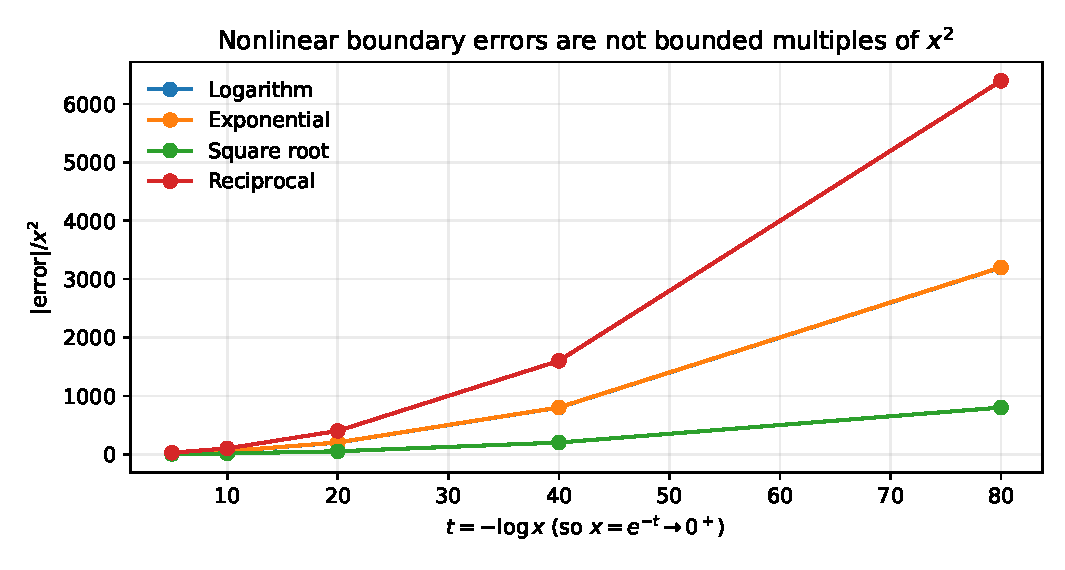
\includegraphics[width=0.96\textwidth]{nonlinear-witness.pdf}
\caption{Independent high-precision evaluations of the four exact functions in F01, not executions of the Wolfram package. The normalized errors grow quadratically in $-\log x$.}
\end{figure}

\textbf{Fix.} When the input precision is active, retain both the input error degree and the generated Taylor-boundary degree. The patch replaces the three-way branch by
\begin{lstlisting}
If[less[cut, PU], {c, Nn d}, {c, Max[Nn d, DU]}]
\end{lstlisting}
with the helper's existing definitions $N_n=\lceil c/\val(U)\rceil$ and $d=\max\deg_L U$. Empty jets and exact infinite precision retain their preceding special cases. This is the conservative rule in \eqref{eq:unitbound}. A later optimization may compute the actual complete boundary block and obtain a smaller degree; it must never replace that with the input degree merely because the requested order is larger.

\textbf{Regression principle.} Test $h<P$, $h=P$, and $h>P$ for the same operand. The known finite coefficients below the common precision should agree, and no boundary logarithm may disappear when a higher cutoff is requested. A useful metamorphic property is that increasing a requested cutoff without refining the operand cannot create a stronger claim by forgetting a generated boundary contribution.

\finding{F02}{Fractional powers of pure remainders bypass the real-branch check}{source-established branch-contract defect}
\label{sec:f02}
\textbf{Location.} The empty-jet branch of \code{fwdPower}. Nonnegative integer powers are handled earlier. For an empty finite jet and a positive noninteger exponent, the function returns a transformed magnitude bound immediately, before its ordinary positive-leading-coefficient test.\cite{repo-core,repo-ops}

\begin{lstlisting}
Clear[x];
s = AsymptoticExpansion[-x, {x, 0, 0}];
SeriesPower[s, 1/2]
\end{lstlisting}
Here the retained finite expression is zero and the error is of order $x$. That magnitude statement says nothing about the sign of the represented function. The stored explicit source is negative on the selected positive side. Its Wolfram principal square root is imaginary, and it has no real square root there. Nevertheless, the inspected empty-jet branch predicts acceptance of a pure $\OO(x^{1/2})$ result without a real-domain proof.

The transformed \emph{absolute magnitude} is not the problem: $|\sqrt{-x}|=\sqrt{x}$ is indeed of that order. The problem is accepting it in an interface whose noninteger-power operations otherwise require a real positive branch. The error class has been used as though it also certified the function's domain.

\textbf{Fix.} Distinguish three cases: exact zero, a nonnegative integer power, and a finite-precision pure remainder with a noninteger power. Exact zero may be raised to a positive exponent. Integer powers are already safe algebraically. The remaining case must either carry an independently proved nonnegative germ sign or fail with a message instructing the caller to refine the operand or supply admissible sign information. The supplied patch chooses the conservative rejection; it does not invent a sign from a magnitude bound.

\textbf{Why inspecting the original source is not automatically the best patch.} Some derived objects represent an error family or a composite operation, not a readily evaluable exact source. Re-entering arbitrary source simplification inside a low-level power primitive introduces expensive and context-sensitive recursion. A better long-term representation stores an optional proof of eventual positivity as a capability. The primitive consumes that proof; a higher-level refinement or domain analyzer may produce it.

\textbf{Tests.} Cover an exact zero, a positive pure remainder, a negative pure remainder, a sign-indefinite unknown remainder, and positive/negative integer and noninteger exponents. Rejecting an unproved positive case is conservative and acceptable; silently claiming a real branch of a negative case is not.

\finding{F03}{The SeriesData property is not a bound-preserving export}{source-established interoperability defect}
\label{sec:f03}
\textbf{Location.} \code{makeSeriesData} and \code{makeInverseSeriesData}. Both inspect the remainder power but omit the remainder's logarithmic degree when constructing a native \code{SeriesData}.\cite{repo-core}

\begin{lstlisting}
Clear[x];
s = AsymptoticExpansion[x + x^2 Log[x], {x, 0, 2}];
{s["Remainder"], s["SeriesData"]}
\end{lstlisting}
The package's bound is explicitly $\OO(x^2\M(x))$. The source trace constructs the native object
\begin{lstlisting}
SeriesData[x, 0, {1}, 1, 2, 1]
\end{lstlisting}
It displays a finite part $x$ and a power-order tail at $2$, with no place for the extra logarithmic degree. If the exported object is read as preserving the package's analytic bound, it has become the stronger and false claim $\OO(x^2)$. The actual error divided by $x^2$ is $\log x$.

This finding should be phrased carefully. It is not an assertion that native \code{SeriesData} is defective or that all native logarithmic series are invalid. Native series arithmetic has its own formal order conventions and can contain logarithmic coefficients. The issue is converting from an explicitly stated analytic error class to a representation that does not retain that class, without marking the conversion as lossy. The documentation of \code{SeriesData} describes a coefficient sequence on a rational exponent lattice, not an extra independent logarithmic error-degree field.\cite{wl-seriesdata}

\textbf{Fix.} The simplest sound policy is to return \code{Missing["LogarithmicRemainder"]} whenever the remainder degree is nonzero. An explicitly requested lossy formal export could be offered separately, but should not masquerade as the same error contract. Another option is an explicit exponent-loss conversion: for any fixed $\epsilon>0$,
\[
 x^\rho\M(x)^d=\OO(x^{\rho-\epsilon}).
\]
The API must record that weakening, select a rational lattice deliberately, and check that retained terms are compatible with the new boundary. Silently changing the exponent would be confusing as well.

The inbound special-function importer already follows this philosophy by weakening an unqualified native tail before proving a sharper bound. Export and import should share one documented precision-conversion policy. A round-trip test should verify that analytic precision never becomes stronger solely because the representation changed.\cite{repo-native}

\finding{F04}{An optional eager native export can dominate memory usage}{source-established resource defect}
\label{sec:f04}
\textbf{Location.} Both native-series exporters compute an LCM of rational exponent denominators and allocate \code{Table[0,{nmax-nmin}]} before the generalized result is returned. This allocation is not controlled by the sparse term budget.\cite{repo-core}

Consider the family
\begin{lstlisting}
AsymptoticExpansion[x^(1/q) + x, {x, 0, 1}]
\end{lstlisting}
for a positive integer $q>1$. There is one retained block, at exponent $1/q$, and one omitted block, at exponent $1$. The native rational lattice has denominator $q$, minimum index $1$, and maximum index $q$. Its allocated coefficient-vector length is therefore
\begin{equation}
 N_{\rm dense}=q-1.
\end{equation}
With $q=10^9$, this requests $999{,}999{,}999$ entries from a tiny sparse expression. No such allocation was attempted in this audit. The size follows exactly from the inspected code. A byte estimate would depend on Wolfram's actual representation; the entry count alone establishes the problem.

The important design flaw is that this is eager work for an optional interoperability property. A caller requesting a generalized sparse expansion pays the full dense conversion cost even when it never reads \code{s["SeriesData"]}. Raising or lowering a sparse \code{MaxTerms} setting does not express an appropriate bound on that dense lattice.

\textbf{Immediate fix.} Before allocating, check the exact dimension against a separate cap and return a descriptive \code{Missing} value rather than failing the entire sparse result. The supplied patch uses an interim cap of $100{,}000$ coefficient entries. That fixed cap is intentionally a stopgap, not a proposed permanent global policy.

\textbf{Preferred design.} Make native export an explicit or lazy operation with \code{MaxDenseEntries} and possibly \code{MaxExportBytes}. Its preflight should report the lattice denominator, vector length, retained nonzero blocks, and why conversion was refused. A non-rational exponent should remain a normal ``not representable in this format'' outcome rather than an error in the generalized expansion itself.

\textbf{Tests.} Check sparse inputs whose exponents have large coprime denominators; a small visible term count does not bound their LCM. Include negative weights and inverse exports. Test the cost estimator without allocation, then use moderate denominators for native smoke tests. The bundled regression uses $q=100003$ under additional time and memory limits so it can safely expose the missing guard on an unmodified checkout.

\finding{F05}{Refinement uses a heuristic forward order rather than a backward demand calculation}{source-established goal-underdelivery defect}
\label{sec:f05}
\textbf{Location.} The ordinary derived-recipe branch of \code{SeriesRefine} in \code{SeriesOperations.wl}. It refines operands using a heuristic based on the requested output cutoff plus a small guard and the operand's stored remainder power, then replays the operation. That request does not generally account for a singular observable's precision loss.\cite{repo-ops}

A useful reproduction candidate is
\begin{lstlisting}
Clear[x];
s = SeriesPower[
  AsymptoticExpansion[Sin[x^10], {x, 0, 21}], -1];
t = SeriesRefine[s, 20];
{Normal[t], t["RemainderPower"]}
\end{lstlisting}
The initial source expansion is
\[
 \sin(x^{10})=x^{10}+\OO(x^{30}),
\]
so its reciprocal is known only as $x^{-10}+\OO(x^{10})$. The replay heuristic requests a source cutoff of $22$ for the desired output cutoff $20$. This still retains just $x^{10}$ and leaves a source remainder at $30$, so the reciprocal remains known only to power $10$. The result may be a valid expansion, but it has not met the refinement request.

The exact reciprocal series makes the missing information explicit:
\[
 \frac1{\sin(x^{10})}
 =x^{-10}+\frac{x^{10}}6+\frac{7x^{30}}{360}+\cdots.
\]
A successful refinement to cutoff $20$ must include $x^{10}/6$, or clearly return a goal-not-reached result. The supplied independent check verifies these coefficients by substituting $z=x^{10}$ into the ordinary expansion of $1/\sin z$.

\textbf{Correct demand transport.} For $f\sim a u^\alpha$ and a fixed power $r$, an input error of power $P$ becomes an output error of power
\begin{equation}
 P+\alpha(r-1).
 \label{eq:power-demand}
\end{equation}
Thus an output target $h$ needs input precision at least $h-\alpha(r-1)$, subject to boundary log degrees and branch hypotheses. Here $\alpha=10$, $r=-1$, and $h=20$, giving $P\ge40$. A fixed ``plus two'' guard cannot substitute for this calculation.

\textbf{Fix.} Introduce a backward precision planner, followed by a forward verification of the achieved result. For multiplication, demand on one operand depends on the valuation of the other. For composition, it depends on the inner valuation and the outer derivative scale. For logarithm, require enough relative rather than absolute precision. For exponential, require a vanishing absolute phase error before converting it to a relative amplitude error. If the requested precision cannot be reached, return a structured failure containing the best valid expansion, the requested bound, the achieved bound, and the blocking operand.

This is distinct from F01. F01 can assert a false error class; F05 can return a true error class that is insufficient for a requested computation. Both matter to a pipeline, but they should not be conflated. The included core patch does not repair this planner; the corresponding native test intentionally remains a target for further implementation.

\finding{F06}{Grouped and Newton inversion can be blocked by direct multi-index enumeration}{source-established performance/architecture limitation}
\label{sec:f06}
\textbf{Location.} The public inverse orchestration in the main kernel, especially construction of \code{indexRegion} and the shared frontier, together with the otherwise genuinely grouped and Newton implementations in \code{IncrementalInverse.wl}.\cite{repo-core,repo-incremental}

For a fixed requested exponent cutoff, the code constructs a multi-index region even when the requested coefficient algorithm is \code{"GroupedLagrange"} or \code{"Newton"}. The region is then used in shared coefficient/frontier logic. Consequently these methods cannot always realize their natural advantage on models with many resonant gaps: they may hit the direct enumeration budget before the grouped/Newton calculation becomes the dominant work.

Take the exact model
\[
 f(x)=x(1+x+x^2+\cdots+x^{20})
\]
and request an inverse cutoff of $42$. The relative correction cutoff is $41$ and the gaps are $1,2,\ldots,20$. The number of nonnegative multi-indices satisfying
\[
 \sum_{j=1}^{20}j k_j<41
\]
is \textbf{207,042}, whereas there are only \textbf{41 distinct weights}, $0,\ldots,40$. The count was computed independently by the coefficient recurrence for
\[
 \prod_{j=1}^{20}(1-z^j)^{-1}
\]
through degree $40$. This is a count of mathematical objects, not a Wolfram timing measurement. It is already over ten times the default $20,000$ index budget, without counting any extra boundary nodes.

\begin{lstlisting}
AsymptoticInverse[
  x Total[Table[x^j, {j, 0, 20}]], {x, 0}, {y, 42},
  Method -> "GroupedLagrange", "MaxTerms" -> 20000]
\end{lstlisting}
The source path predicts an enumeration-budget failure, even though the grouped representation has a much smaller support. This does not imply every grouped request fails or that merely switching methods guarantees a fast computation; coefficient growth and convolution costs still matter.

\textbf{Fix.} Dispatch the coefficient algorithm before choosing its work representation. A grouped method should obtain a certified cutoff error and, when affordable, its first omitted complete weight from grouped support calculations. Newton should certify its requested precision from its residual and model error, without requiring an exhaustive direct-index frontier. If a sharp first omitted block costs too much, return a conservative bound at the requested cutoff and mark the sharper frontier unavailable. Optional diagnostic sharpness should not defeat the selected algorithm.

A separate complete-index mode remains valuable for \code{InverseExpansionCoefficient} and explicit multi-index provenance. It need not be mandatory for all inverse computations. The algorithm should report whether cost was spent on coefficient generation, exact ordering, frontier discovery, or provenance.

\textbf{Additional local optimization.} The incremental state currently selects all boundary entries at the next weight and sorts the remaining boundary to find the next minimum. A persistent exact-weight priority queue can reduce repeated whole-boundary scans. Canonical equality and collision completeness must be preserved: it is not safe to pop one node and declare a weight complete before all its equal-weight contributions are available.\cite{repo-incremental}

\finding{F07}{The flat-rate parser implements a stricter condition than commensurability}{source-established missing supported case}
\label{sec:f07}
\textbf{Location.} \code{flatModel} in \code{FlatSectors.wl}. It chooses the smallest input rate as the fundamental rate and requires every other rate divided by that rate to be an integer.\cite{repo-flat}

For example,
\begin{lstlisting}
AsymptoticFlatInverse[
  x + Exp[-2/x] + Exp[-3/x], {x, 0}, {y, 3}]
\end{lstlisting}
has commensurate rates $2$ and $3$, with natural marker $E=e^{-1/x}$ and input sectors $E^2$ and $E^3$. The current test uses base $2$, finds the ratio $3/2$, and rejects the expression as incommensurate. There is no mathematical obstacle to representing it in the existing one-marker polynomial algebra.

\textbf{Fix.} Choose any positive reference rate $c_*$ and prove that the ratios $r_j=c_j/c_*$ are rational. Set
\[
 D=\operatorname{lcm}(\operatorname{den}r_j),\qquad
 n_j=Dr_j,\qquad g=\gcd(n_1,\ldots,n_m).
\]
Then the fundamental rate and sector degrees are
\begin{equation}
 c_0=c_*g/D,\qquad d_j=n_j/g.
 \label{eq:flatgcd}
\end{equation}
This handles rates $2,3$ with $c_0=1$ and degrees $2,3$, and rates $2/3,4/5$ with $c_0=2/15$ and degrees $5,6$. It also handles a common irrational factor when exact ratio simplification proves rationality.

The optional patch implements this scalar rational-lattice normalization and preflights the largest resulting sector degree against the existing budget. The preflight is essential: close rational rates may yield an extremely fine fundamental lattice and a large marker degree. An eventual sparse sector map would avoid allocating all missing degrees, but would still need a work budget.

With the new marker, the example's inverse through sector degree three is simply
\[
 y-e^{-2/y}-e^{-3/y}.
\]
The first cross/self-correction starts at degree four. A constructor should record the chosen generator because an inclusive sector depth is meaningful only relative to that generator. Truly irrationally related rates require a multi-generator extension; they are not fixed by the scalar gcd calculation.

\section{Algorithmic and performance analysis beyond the concrete defects}
\label{sec:performance}
\subsection{The inversion formula and where work is duplicated}
For \eqref{eq:model}, put $w=\sum_j k_j\delta_j$ and $n=\sum_j k_j$. The nonzero multi-index contribution to the normalized observable $u^r$ is generated by
\begin{equation}
 C_{\boldsymbol k}(L)=
 \frac{(-1)^n r}{p^n\prod_j k_j!}
 \left[\prod_{\ell=1}^{n-1}
    \left(\frac{d}{dL}+r+w+p\ell\right)\right]
 \prod_j B_j(L)^{k_j}.
 \label{eq:lagrange}
\end{equation}
The inverse term is $z^{r+w}C_{\boldsymbol k}(\log z)$, and the zero multi-index supplies the leading $z^r$. This is the operator formula visible in the ordinary and incremental implementations. For $p=r=1$, one gap $1$, and $B=1$, it gives the familiar first correction coefficients $-1,2,-5$ for the inverse of $x+x^2$.\cite{repo-core,repo-incremental}

The grouped implementation exploits a real algebraic fact: at fixed $(n,w)$ the Euler operator in \eqref{eq:lagrange} is identical. Computing the coefficient of weight $w$ in the $n$th power of the perturbation automatically combines the multinomial factors, replacing separate $\prod k_j!$ denominators with $n!$. This is not merely caching. It changes the objects over which the algorithm iterates. The public work scheduler should honor that change, as discussed in F06.

\subsection{Existing optimizations should not be rediscovered as missing features}
The ordinary sparse product already uses sorted support and skips columns beyond an exclusive cutoff. Nonnegative integer powers already use binary powering in the precision algebra. Fourier powers also use binary powering, and Fourier source-weight multiplication similarly skips inadmissible columns. Incremental inversion already caches powers of logarithmic polynomials with a capacity policy that yields to the index budget. Newton already uses precision doubling and an exact finite-model residual check. Recommendations should therefore focus on the remaining bottlenecks rather than propose these existing features as absent.\cite{repo-core,repo-fourier,repo-incremental}

Several opportunities remain. Gamma inverse coefficient construction repeatedly asks native \code{Series} for increasingly high orders while growing the unit correction; a persistent truncated polynomial representation or coefficient-by-coefficient recurrence can avoid repeated reconstruction. The native importer's positive integer-power branch uses repeated multiplication rather than the core's binary-power primitive. General \code{Expand}, \code{Together}, \code{Simplify}, and \code{FullSimplify} calls remain candidates for profiling before any broad rewrite. These are proposed performance experiments, not measured bottlenecks in this environment.\cite{repo-gamma,repo-native,repo-core}

\subsection{State size, cache semantics, and exact ordering}
The incremental state is returned by value and does not leave a process-global coefficient cache. That makes failed refinement easier to reason about. However, repeated association and list reconstruction, string keys for multi-indices, full boundary scans, and polynomial expression growth can still create large transient allocations. Store counters for candidate indices, distinct weights, canonicalization calls, coefficient terms, and cached polynomial sizes so that a resource failure is diagnosable.\cite{repo-incremental}

A safe cache key must include the effective assumptions and coefficient domain, not just the printed expression. A comparison proved under $a>0$ cannot be reused under an unrelated parameter regime. For algebraic exponents, a canonical algebraic representation and cached comparisons may be effective. For broader exact numeric expressions, failure to prove an order must remain a possible outcome.

\textbf{Unconfirmed comparator risk.} The low-level comparison fallback can interpret a simplified false result for $a-b<0$ as positivity after an earlier equality attempt. Logically, ``not negative'' also includes zero. Without a concrete public witness this is a code-hardening concern, not an additional demonstrated wrong answer. Replace the fallback by explicit proof attempts for $a-b<0$, $a-b>0$, and $a-b=0$, and return \code{UndecidableOrder} if none is established. Exact ordering underlies collision grouping and should not depend on an unproved trichotomy branch.\cite{repo-core}

\subsection{MaxTerms conflates several resource dimensions}
Depending on the engine, \code{MaxTerms} bounds retained pairs, candidate pairs, multi-indices, expression leaves, iteration counts, or stored coefficient support. Those quantities are correlated only loosely. A budget of $20,000$ means different feasible problems in different methods. Some time constraints are local fixed values rather than a deadline for the entire public operation. A sequence of many individually bounded symbolic calls can therefore exceed a user's expected total time by a large factor.\cite{repo-core,repo-envelope,repo-native,repo-fourier}

Introduce a request-level work context with distinct counters and a shared deadline. At minimum, separate maximum support size, candidate convolution pairs, coefficient-expression size, native-series working order, dense-export size, Fourier frequencies, and symbolic subcall time. Return the consumed and required quantities in a resource failure. Reusing \code{MaxTerms} as a compatibility shorthand is reasonable, but the internal budget must have a precise unit.

\subsection{How to read the repository's timing claims}
The 1.8.0 validation record reports focused microbenchmarks, including substantial improvements to coordinate inversion, Fourier grouping, and a truncated Fourier product. It also reports a much smaller change for a public Fourier inverse. Earlier records include examples with little overall improvement or variable timings despite a large local speedup. These are useful records precisely because a local primitive speedup is not automatically an end-to-end speedup.\cite{repo-validation}

The latest commit record reports 305 tests in 18 focused files, seven standalone checks, and eleven Python builder tests, while explicitly saying that the full Wolfram suite was not run for that change. Do not add historical counts from different commits and call the sum a current passing suite. The CI workflow inspected here verifies generated standalone freshness and runs the Python builder tests; it is not a native Wolfram mathematical regression job.\cite{repo-validation,repo-ci}

\section{API and user-experience issues}
\label{sec:api}
\subsection{One numeric argument denotes many different notions of order}
The user guide does explain the order conventions, including an extensive table. The problem is therefore not missing documentation; it is that the public syntax makes semantically different quantities look interchangeable. An ordinary cutoff is an exclusive exponent bound. A flat depth is an inclusive marker degree. A Gamma inverse cutoff is in powers of the reciprocal core. A structured native special-function term goal applies separately to each carrier, so the total displayed block count can exceed that goal. A depth-truncated symbolic expansion may not be ordered at all.\cite{repo-guide}

Introduce a normalized request object internally and optionally a clearer explicit public form, for example:
\begin{lstlisting}
<|"GoalType" -> "ExponentCutoff", "Value" -> 5,
  "Coordinate" -> "RecordedLocalCoordinate",
  "Boundary" -> "Exclusive"|>

<|"GoalType" -> "CompleteBlocks", "Value" -> 5,
  "Scope" -> "PerCarrier"|>

<|"GoalType" -> "SectorDepth", "Value" -> 3,
  "Boundary" -> "Inclusive", "RateGenerator" -> 1|>
\end{lstlisting}
The familiar short forms can remain as convenience syntax. Every returned object should expose the normalized request, its actual achieved precision, and a Boolean or structured explanation of whether the goal was reached. A remainder beyond a requested cutoff is a successful stronger result; a remainder before it needs an explicit explanation.

\subsection{The result head is unified, but its capabilities are not}
Version 1.8.0 deliberately replaces \code{PowerLogSeries} with \code{GeneralizedSeries}, and the guide tells users to update explicit patterns and saved inputs. This is a sensible name for the current range of scales. It is nevertheless a serialization migration: a saved expression contains the old head and an association whose schema may also evolve. A versioned schema and an explicit migration utility would be safer than relying only on pattern replacement.\cite{repo-guide,repo-commit}

A property such as \code{"RemainderPower"} is not a universally comparable measure across different prefactors and coordinates. Similarly, the presence of \code{"Model"} or \code{"Terms"} is not enough to conclude that a generic coefficient extractor or composition operation applies. Add stable capability queries such as ``ordered power-log algebra'', ``source replay'', ``inverse model residual'', ``derivative contract'', ``native export'', and ``pointwise certificate''. Operation dispatch can then reject unsupported combinations before accessing missing or semantically unrelated association keys.

A validation function for result objects should check coordinate consistency, sorted merged support, the relation between kept terms and the error boundary, domain metadata, and the declared scale. This is useful for debugging and persisted results; it need not attempt to treat ordinary Wolfram expressions as a secure unforgeable data type.

\subsection{Numeric evaluation is a finite approximation, not a bound}
The current \code{s[value]} implementation substitutes into the stored finite expression. The guide explicitly says so, and \code{Normal[s]} explicitly drops the remainder. Neither behavior is intrinsically wrong. However, the visually attractive series display can encourage a user to regard numeric evaluation as a controlled approximation at any supplied point. A Poincar\'e remainder with an existential constant and threshold does not provide that assurance.\cite{repo-core,repo-guide}

Retain the convenience operation but add a separate \code{SeriesEvaluate} returning the finite value, target-domain status, remainder scale, effective numerical precision, and evidence type. It should distinguish ``asymptotic scale only'' from ``certified bound at this target''. An optional domain check is useful; a numerical error estimate must not silently assume the big-$O$ constant is one. The existing inverse numerical checker already substitutes exact targets before numerical evaluation and checks source conditions at the recovered source root. That practice should be reused.\cite{repo-numeric}

The legacy field \code{"ExactInverse"} in a numerical check is especially easy to misuse, even though the code documents it as an alias of \code{"ReferenceRoot"}. Prefer the latter in new output and eventually deprecate the former. A \code{SourceDomainVerified -> True} flag in a floating-point report should travel with an explicit evidence classification; the same wording in a rational certificate has a stronger meaning.\cite{repo-numeric,repo-cert}

\subsection{Power means a centered observable at a finite endpoint}
For an ordinary inverse at a finite source endpoint $x_0$, \code{"Power" -> r} with $r\ne1$ requests $(x-x_0)^r$, while $r=1$ reconstructs the original source variable including $x_0$. At infinity it denotes $x^r$. This convention is documented and should not be called an implementation bug. It is, however, a discontinuity in the meaning of the option at $r=1$.\cite{repo-guide}

A future interface can separate the observable from the coordinate, for example \code{Observable -> Function[x, x^r]} or a named centered-coordinate observable. It should be possible to inspect both the source root and the requested observable without reversing the meaning of a power option. Compatibility syntax can retain the existing behavior with an unambiguous normalized observable field.

\subsection{Assumptions, holding, and replay deserve explicit policy}
The package's public defaults advertise \code{Assumptions -> True}, whereas several native asymptotic interfaces advertise \code{$Assumptions}. It would be unsafe to infer that all uses of \code{Assuming} are equivalent across these APIs. Native subcalls may also have their own ambient assumption behavior. Normalize the effective assumptions once, retain them on the result, and consistently pass them into every proof and canonicalization operation. Tests should cover both explicit assumptions and ambient \code{Assuming}, including parameter conditions and conditions on the source variable.\cite{repo-guide,wl-asymptotic,wl-series}

The held public entry points support expressions and callable inverses, and the guide asks callers to leave source and target symbols unassigned. These choices help preserve branch syntax, but should be tested against assigned symbols, nested \code{ConditionalExpression}, pure-function scoping, and definitions that change after a result is constructed. Retain both an inert source description and the normalized model used for the original calculation, so a replay failure can say whether definitions or assumptions changed rather than appearing to refine the same immutable mathematical object.

\subsection{Automatic arithmetic should not hide capability changes}
Ordinary \code{Plus}, \code{Times}, \code{Power}, and selected unary functions dispatch through upvalues. Unsupported common ordered scales may fall back to composite error envelopes. This is often useful: a valid absolute bound is better than refusing every mixed-scale sum. But a caller may inadvertently lose ordered composition, inverse residual, or refinement capabilities after such a fallback. The result should identify the operation that caused the transition and the capabilities that remain.\cite{repo-arithmetic,repo-envelope,repo-guide}

The held \code{SeriesNormalize} route is particularly valuable where ordinary evaluation could cancel or simplify a denominator before the package sees a singularity. Document this as an evaluation-semantics issue rather than suggest that every expression involving a generalized series has exactly native \code{SeriesData} semantics. Test both held normalization and ordinary arithmetic on the same potentially singular expressions.

\section{Validation that would catch these defects}
\label{sec:testing}
\subsection{Regression tests should target boundaries, not just coefficients}
The inspected \code{SeriesOperations.wlt} already tests common precision transport, a reciprocal's loss of absolute precision, ramified composition, wrong-limit rejection, complete boundary log degree on truncation, source replay, derivative-contract rejection, and compatible variables. These are valuable tests. The missing pattern exposed by F01 is more specific: an \emph{already truncated logarithmic operand}, followed by a nonlinear operation requesting a cutoff strictly beyond the operand's known precision.\cite{repo-tests}

A compact boundary matrix should vary the requested cutoff below, at, and above the known precision; coefficient log degree zero and positive; empty, constant-leading, and singular-leading jets; finite endpoints on both sides; positive and negative infinity; exact input and declared input error; and exact cancellation at the first candidate boundary. This matrix tests the error calculus rather than merely comparing printed coefficients.

\subsection{Useful metamorphic properties}
Several properties can be checked without a huge reference database. Truncating twice should agree with the more restrictive compatible truncation. Compatible translations and reciprocal coordinate changes should commute with reconstruction. All ordinary inversion methods should give the same complete coefficients below a common certified cutoff. Refinement followed by truncation should recover the original known coefficients and should not erase original source conditions. A native export/import round trip must never strengthen an analytic error claim. Raising a work budget must not silently change a failure into an unjustified answer.

For arithmetic, compare a direct expansion of an exact test function with the corresponding operation on an intentionally truncated operand. The two finite parts may differ at the boundary, but the reported errors must enclose their difference in the asymptotic sense. This is the structure used by the independent randomized polynomial checks, and it scales naturally to generated Wolfram tests.

\subsection{Independent oracles and their limits}
For rational exponents on a manageable common grid, substitute $u=t^q$ and use exact polynomial arithmetic or native formal series as a second implementation. For a logarithmic polynomial, temporarily treating $L$ as an independent indeterminate is a valid way to calculate fixed coefficients; the final remainder proof must then restore $L=\log u$. For Lagrange inversion, compare direct multi-index coefficients with grouped coefficients and exact substitution into the finite model. For Gamma and Barnes asymptotics, compare the finite logarithmic residual and its separately justified model remainder, not just the first few coefficients.

High-precision sampling is useful for falsification. It does not prove a uniform statement, and a ratio that appears bounded at a few modest targets can still grow like $\log\log y$. Sample in the actual small coordinate, record that coordinate, and use exact target construction to avoid losing a tiny target distance to a large offset. The existing numerical code already recognizes this last issue.\cite{repo-numeric}

\subsection{Test the proof infrastructure itself}
The interval evaluator deserves separate tests for directed rounding, multiplication across zero, integer powers, reciprocal singularities, logarithmic domain boundaries, exponential range reduction, and exact endpoint contact. Test that every admitted Boolean source condition holds on the entire closed interval, not only at sample points. An exact root at a boundary, a constant derivative close to zero, and an interval with no root should all be represented in the suite.\cite{repo-cert}

For error descriptors, test the distinction between a zero function and a zero retained jet. For Fourier coefficients, test algebraic frequency resonances, conjugate pairing, cancellations before frequency counting, and failure without mode deletion. For flat sectors, test gaps in marker degrees, the exactness of the zero sector, rationally commensurate rates, and failure before a huge normalized lattice is allocated.\cite{repo-fourier,repo-flat}

\subsection{Release gates and reproducibility}
A release that changes the public result head and shared operation internals should have a complete native suite gate in addition to focused development tests. Record the kernel version, system identifier, source commit, canonical source hashes, standalone hash, test-file inventory, elapsed time, resource ceilings, and any excluded tests with reasons. Maintain a small cross-platform matrix and the minimum supported kernel version, because native special-function output shapes are part of this package's effective dependency surface.

The existing standalone CI is useful and should remain. Add native tests through an appropriately provisioned runner rather than assume Python freshness checks exercise mathematical behavior. Also test both loading forms: canonical modular source and generated standalone file. Generated artifacts should be rebuilt from canonical sources, never edited independently.\cite{repo-ci,repo-validation}

\section{Recommendations for future development}
\label{sec:roadmap}
\subsection{Priority 0: protect the meaning of a result}
Merge and natively validate the conservative F01--F04 fixes, add the boundary matrix, and make the known/unknown/empty distinctions explicit. Require that every constructor and operation either returns a valid documented error class or a structured failure. Add an audit assertion mode that checks sorted merged support, coordinate consistency, branch prerequisites, and whether newly discarded terms are covered by the returned bound. Assertions can be disabled in optimized production paths only after tests establish the invariants.

Expose an evidence classification on all result families: exact finite expression; asymptotic expansion with stated hypotheses; finite-model residual check; numerical sample; or pointwise rational certificate. This does not require formal proof-assistant integration. It first requires consistent data and vocabulary.

\subsection{Priority 1: a real precision planner}
Represent precision as a scale-aware bound plus regularity information, not merely an exponent and ad hoc guard. Each operation should implement two functions: a backward demand transformer and a forward achieved-bound transformer. The backward function determines what operands must know; the forward function checks what the actual operands justify. Their agreement should be a testable invariant.

For ordinary powers, use \eqref{eq:power-demand}. For products, require the operand errors to be small compared with the desired output after multiplication by the other operand's leading scale. For composition $F(G(u))$, transport the outer remainder through $G$ and the inner uncertainty through a bound for $F'$. Track log degrees at equal power boundaries. For exponential carriers, preserve absolute phase-error requirements. Once this layer exists, \code{SeriesRefine} can report a reasoned source demand instead of guessing how much additional order might help.

Memoize refinement recipes as a directed acyclic graph where practical. Shared subexpressions should be refined once to the strongest combined demand, rather than copied and replayed repeatedly along different branches. An immutable graph also provides clearer provenance and lets failed refinement preserve the last valid object.

\subsection{Priority 2: decouple algebra, scheduling, and presentation}
Separate the coefficient domain from the support/order structure. An ordinary coefficient domain is a polynomial ring in $L$; a Fourier domain adds a finite exact frequency map; Gamma inverse coefficients use polynomials in a reciprocal logarithm. Each domain should provide exact addition, multiplication, differentiation, equality testing under assumptions, and a conservative absolute envelope. The support layer should provide exact ordered weights, convolution under a cutoff, and complete boundary grouping. The scheduler should select direct, grouped, or Newton work independently of formatting and optional frontier presentation.

Make native-series export lazy or explicit. Introduce a capability registry for family dispatch rather than spreading all support knowledge across string-valued scale tests and load-order-dependent private definitions. Preserve detailed failure reasons when an optimized ordered route falls back to an envelope, so performance and capability regressions are visible.

\subsection{Priority 3: integration of supported generalized germs}
The absence of a general public integration operation is a practical extension opportunity. It should complement, not replace, native \code{AsymptoticIntegrate}, whose scope includes integral asymptotics such as Laplace and oscillatory methods. A first repository implementation can integrate its own already-constructed power--log germs, with explicit anchoring and error conditions.\cite{wl-integrate,repo-guide}

For a polynomial $P$ and $\alpha\ne-1$, seek a polynomial $Q$ satisfying
\[
 Q'(L)+(\alpha+1)Q(L)=P(L).
\]
Then
\[
 \int u^\alpha P(\log u)\,du=u^{\alpha+1}Q(\log u)+C.
\]
The polynomial equation is triangular in degree and can be solved exactly. At the resonance $\alpha=-1$, integrate $P(L)$ directly in $L$. For a remainder integrable from zero, $\OO(u^\rho\M^d)$ with $\rho>-1$ integrates to $\OO(u^{\rho+1}\M^d)$. The critical exponent and nonintegrable cases require a different anchor or additional information. Coordinate changes at infinity must include their Jacobian. These are finite, explicit contracts suitable for the same assertion and test infrastructure.

\subsection{Priority 4: broader logarithmic coefficient algebras}
The ordinary leading-coefficient restriction is a natural boundary. A leading $u^p P(\log u)$ with nonconstant $P$ often requires reciprocal or iterated logarithmic scales rather than another power-log polynomial. Extend this by explicit coefficient fields and transformations, not by silently allowing an unsupported leading logarithm into ordinary division.

One useful intermediate target is rational functions of $\log u$ with a proved nonvanishing denominator on the approach, together with an explicit expansion coordinate $1/\log u$. Another is a finite nested hierarchy $\log u$, $\log(-\log u)$, and so on, where each step records its own dominance and domain facts. Generic composition then needs a justified scale transformation, not merely expression substitution.

\subsection{Priority 5: sparse multi-generator sectors}
F07 can be fixed without a general transseries engine. A broader extension could store flat sectors by a vector of nonnegative generator indices and use exact dominance of the associated phase functions. Equal phase powers with irrationally related rates can then share the existing exact-weight machinery; different phase powers require a hierarchical dominance policy. Sector cutoffs and coefficient cutoffs should remain separate, and an algebraic approximation must never be declared an exact zero sector just to make a representation fit.

A general complex-sector and Stokes-aware system is a much larger project than extending a real rate lattice. It needs sector domains, phase comparisons, branch continuation, and a precise statement of which exponentially small information is retained. There is no reason to promise that as a quick consequence of recognizing more special-function heads. Native complex asymptotic interfaces are already a broader baseline in that direction.\cite{wl-asymptotic,wl-asymptoticsolve}

\subsection{Gamma and Barnes inverses: retain the useful hierarchy}
For a large Gamma target, set $T=\log y$ and
\[
 X=\frac{T}{W(T/e)}.
\]
Then $X(\log X-1)=T$. The finite Stirling model leads naturally to
\[
 x=X+\frac12-\frac{\log(2\pi)}{2\log X}+\cdots,
\]
with complete polynomials in $1/\log X$ at each subsequent inverse power of $X$. For Barnes $G$, the corresponding core is
\[
 X=\sqrt{\frac{4T}{W(4T/e^3)}},
\]
solving $\tfrac12X^2\log X-\tfrac34X^2=T$, and the coefficient variable is $1/(\log X-1)$. These identities follow directly from the defining equation of $W$ and the leading logarithmic Gamma/Barnes asymptotics. The code uses finite Poincar\'e models rather than claiming their infinite asymptotic series converge.\cite{repo-gamma,wl-productlog,dlmf-gamma,dlmf-barnes}

This hierarchy is worth preserving. Expanding $W$ into nested logarithms too early can turn one exact core plus short coefficient polynomials into a much larger expression and obscure ordering. Development effort should instead improve incremental coefficient construction, precision-demand transport, generic operations that respect this coefficient scale, and independently checkable finite-model remainder records. The guide correctly distinguishes these ordered inverse families from the separate perturbative special-inverse adapters; their integer order arguments are not interchangeable.\cite{repo-guide,repo-gamma}

\subsection{Machine-checkable proof records}
A longer-term direction is to export small local proof obligations rather than a single unstructured claim that a result is ``verified''. Examples include a canonical polynomial identity for a grouped coefficient; a finite-model residual vanishing below a cutoff; a coordinate map and its derivative; a nonzero leading-sign condition; an error-transport rule with its operand bounds; and rational interval endpoints with outward-rounded arithmetic steps.

A lightweight independent checker can initially validate the rational and polynomial portions. More sophisticated checks may trust native algebraic normalization or interval routines explicitly. This architecture makes the trusted boundary visible and allows later formal verification without requiring the entire front-end expression recognizer, simplifier, and notebook formatter to be verified at once.

\section{Using the accompanying artifacts}
\label{sec:artifacts}
\subsection{Independent checks}
From the archive root, run:
\begin{lstlisting}
python -m pip install -r code/requirements.txt
python code/verify_counterexamples.py
python -m unittest discover -s code -p test_patch_tools.py -v
\end{lstlisting}
The first program writes exact-check details and high-precision witness ratios into \code{results/}. The optional \code{plot_witness.py} rebuilds the included figure and requires matplotlib. The supplied figure is already present, so rebuilding the article does not require rerunning Python. These checks establish the mathematics and helper behavior described in this review, not native execution of the package.

\subsection{Patch application}
The patcher defaults to a dry run and checks the pinned Git blob hash of each canonical file before matching exact source fragments. The optional flat-rate extension affects an additional file. On a local checkout:
\begin{lstlisting}
python patches/apply_review_patches.py /path/to/Asymptotic
python patches/apply_review_patches.py /path/to/Asymptotic \
  --include-flat-lattice

# After inspecting the diff:
python patches/apply_review_patches.py /path/to/Asymptotic \
  --include-flat-lattice --write

# From that repository root, rebuild the generated standalone file:
python validation/build_standalone.py
\end{lstlisting}
Existing sources are backed up before replacement. The patcher refuses unrelated versions and refuses to overwrite a pre-existing backup. It does not modify the root generated package directly. F01--F04 are included; F07 is optional. F05 and F06 require the planner and scheduler work described earlier and are not claimed to be fixed by this patch.

The fixed dense-export cap is an interim policy, and the pure-remainder branch fix is deliberately conservative. A maintainer may prefer explicit export budgets and stored positivity proofs. Either refinement should preserve the contracts established here. No natively tested patched release is being asserted.

\subsection{Native tests and comparison}
Set the environment variable \code{ASYMPTOTIC_REPO} to a local checkout and run \code{code/RunNativeAudit.wl} in a fresh Wolfram kernel. For example, on PowerShell:
\begin{lstlisting}
$env:ASYMPTOTIC_REPO = 'C:\src\Asymptotic'
wolframscript -file code/RunNativeAudit.wl
wolframscript -file code/CompareBuiltins.wl
\end{lstlisting}
The test file contains twelve candidates. Some are expected to fail on the reviewed baseline; F05 and F06 remain implementation targets even after the supplied patch. Their tests are not a substitute for the repository's full native suite. The runner records the kernel version, system identifier, source hash, and test summary. The comparison runner records raw results before any claim of capability or performance parity is made.

Native output files are intentionally absent from the supplied results directory. \code{native_status.json} records that no native run occurred, rather than presenting empty or invented pass counts. This is important when the archive is later used as input to another review.

\subsection{Article build}
The article uses a standard pdfLaTeX toolchain and included vector figure:
\begin{lstlisting}
cd article
latexmk -pdf -interaction=nonstopmode -halt-on-error \
  asymptotic-review.tex
\end{lstlisting}
The bibliography is embedded in the \code{.tex} source. No font files are distributed in the archive; a TeX installation supplies its own fonts and packages.

\section{Conclusion}
The repository's strongest direction is an inspectable, real-branch-aware generalized asymptotic algebra that cooperates with Wolfram's existing symbolic engines. Its ordinary inverse machinery, exact logarithmic blocks, specialized Gamma/Barnes hierarchies, and explicit evidence distinctions justify that direction. Its broad native special-function support is best understood as a carefully constrained adapter, while native implicit-system, integral, differential-equation, and complex asymptotic facilities remain a broader complementary toolset.\cite{repo-core,repo-guide,repo-native,wl-asymptoticsolve,wl-integrate,wl-dsolve}

The next release should be judged first by whether every displayed remainder, real-branch assertion, refinement goal, and optional conversion means exactly what it says. The concrete findings show where that contract currently breaks or becomes unexpectedly expensive. Conservative repairs are available for the most urgent cases. Precision planning, capability-driven dispatch, and method-specific scheduling then provide a foundation on which broader scale support can be added without multiplying special-case failure modes.

\appendix
\section{Source coverage and traceability}
\label{sec:coverage}
The following table records the scope of this review, not a claim that every file in the repository was executed or line-by-line audited. Function names provide stable navigation anchors within the pinned sources; the GitHub bibliography links select that commit.
\begin{longtable}{@{}p{0.42\textwidth}p{0.50\textwidth}@{}}
\toprule Source or family & Review scope\\\midrule\endfirsthead
\toprule Source or family & Review scope\\\midrule\endhead
\code{Kernel/AsymptoticInverse.wl} & Direct inspection across the main file: primitives, forward/inverse orchestration, precision, export, formatting, model/residual interfaces, and module loading. F01--F04 and F06 are anchored here.\\[6pt]
\code{SeriesOperations.wl}, \code{SeriesArithmetic.wl} & Direct inspection of shared representation conversion, arithmetic and unary dispatch, composition, differentiation, and recipe refinement. F05 is anchored in the replay path.\\[6pt]
\code{SeriesEnvelopeArithmetic.wl} & Selected direct inspection of coordinate/error normalization, compatibility, conservative envelope construction, and resource policy; not every fallback branch independently proved.\\[6pt]
\code{IncrementalInverse.wl} & Direct inspection of incremental frontier state, polynomial cache, coefficient formula, Newton precision doubling, and grouped Lagrange implementation.\\[6pt]
\code{NativeSpecialFunctions.wl} & Direct inspection of tree import/error transport, real projection, coefficient/sector splitting, working-order growth, native backend, and returned contracts.\\[6pt]
\code{InverseCertificates.wl} & Direct inspection of rational arithmetic, exp/log enclosures, domain conditions, root-existence logic, and public refinement/certificate orchestration. No independent proof of all implementation paths is claimed.\\[6pt]
\code{NumericalInverseChecks.wl}, \code{RefinementRequests.wl} & Direct inspection of numerical source/target checks, evidence labels, structured refinement, and tolerance-versus-symbolic-order distinction.\\[6pt]
\code{GammaInverse.wl} & Direct inspection of family recognition, coefficient recurrence, Lambert core, first omitted block, model remainder metadata, and primary construction path.\\[6pt]
\code{FlatSectors.wl} & Direct inspection of phase/rate parsing, exact-core restriction, sector construction, and majorant contract. F07 is anchored here.\\[6pt]
\code{FourierCoefficients.wl} & Direct inspection of coefficient algebra, frequency merging/budget, mode reality, truncated source convolution, and coefficient formula; not a full audit of every downstream Fourier route.\\[6pt]
Lambert, coordinate, reciprocal-log, forward Gamma/Barnes, special-inverse adapters, and remaining dispatch modules & Interface and architecture coverage through main orchestration, imports, guide, and validation record; specialized internal implementations not exhaustively inspected.\\[6pt]
\code{Tests/SeriesOperations.wlt} & Direct inspection of existing arithmetic, composition, derivative, and refinement regression cases. Other suite coverage assessed from validation records, not a complete test-source census.\\[6pt]
Guide, README, validation record, commit, CI workflow & Direct inspection of relevant interfaces, release statements, historical/focused test distinctions, loader/distribution policy, and standalone CI.\\
\bottomrule
\end{longtable}

\section{Independent witness results}
\label{sec:results}
The following are values of exact mathematical test functions evaluated with mpmath at 180 decimal digits. They are not package outputs. Each entry is $(f(x)-A(x))/x^2$ for the retained approximation in F01, with $x=e^{-t}$.
\begin{center}
\begin{tabular}{@{}rrrrr@{}}\toprule
$t$ & Logarithm & Exponential & Square root & Reciprocal\\\midrule
5 & $-11.753198$ & $13.327694$ & $-2.670140$ & $24.800714$\\
10 & $-49.014684$ & $50.991980$ & $-12.002725$ & $99.044512$\\
20 & $-199.000005$ & $200.999997$ & $-49.500001$ & $399.000016$\\
40 & $-799.000000$ & $801.000000$ & $-199.500000$ & $1599.000000$\\
80 & $-3199.000000$ & $3201.000000$ & $-799.500000$ & $6399.000000$\\\bottomrule
\end{tabular}
\end{center}
The exact leading polynomials are $1-t^2/2$, $1+t^2/2$, $1/2-t^2/8$, and $t^2-1$, respectively. For F03, the native-export witness gives the exact normalized error $-t$.

For F06, a 41-entry integer dynamic-programming array gives 207,042 nonnegative multi-indices below weight 41 for gaps $1,\ldots,20$; there are only 41 possible integer weights. For F04, the dense export length for $q=10^9$ is calculated symbolically as $q-1$; no large array is allocated. The randomized boundary checks use a fixed seed and exact rational coefficient arithmetic, and the JSON output records each case's actual and proposed logarithmic degree.

\section{Suggested issue tracker entries}
Use F01--F07 as stable issue labels. Acceptance should enforce contracts: preserve generated boundary degrees; require fractional-power branch evidence; mark or refuse lossy exports; bound dense allocation without losing the sparse result; meet or explicitly fail refinement goals; decouple grouped/Newton execution from direct enumeration; and normalize admitted rational rate lattices subject to a cost bound. Keep comparator hardening and a versioned capability schema as separate design tickets, not reproduced wrong-answer defects.

\clearpage
\begin{thebibliography}{99}
\small
\bibitem{repo-commit} Vladimir Reshetnikov. \emph{Asymptotic repository, reviewed commit and release change}. Commit \commit, 9 September 2026. \url{https://github.com/VladimirReshetnikov/Asymptotic/commit/07a9781212beb2eeb9ff16aa625b50ac27974078}.
\bibitem{repo-core} \emph{AsymptoticInverse/Kernel/AsymptoticInverse.wl}. Main engine at the reviewed commit. \url{https://github.com/VladimirReshetnikov/Asymptotic/blob/07a9781212beb2eeb9ff16aa625b50ac27974078/AsymptoticInverse/Kernel/AsymptoticInverse.wl}.
\bibitem{repo-guide} \emph{AsymptoticInverse User Guide}. Reviewed sections on public functions, result representation, coordinates, orders, arithmetic, Gamma/Barnes inverses, and evidence. \url{https://github.com/VladimirReshetnikov/Asymptotic/blob/07a9781212beb2eeb9ff16aa625b50ac27974078/AsymptoticInverse/Documentation/UserGuide.md}.
\bibitem{repo-ops} \emph{SeriesOperations.wl}. \url{https://github.com/VladimirReshetnikov/Asymptotic/blob/07a9781212beb2eeb9ff16aa625b50ac27974078/AsymptoticInverse/Kernel/SeriesOperations.wl}.
\bibitem{repo-arithmetic} \emph{SeriesArithmetic.wl}. \url{https://github.com/VladimirReshetnikov/Asymptotic/blob/07a9781212beb2eeb9ff16aa625b50ac27974078/AsymptoticInverse/Kernel/SeriesArithmetic.wl}.
\bibitem{repo-envelope} \emph{SeriesEnvelopeArithmetic.wl}. \url{https://github.com/VladimirReshetnikov/Asymptotic/blob/07a9781212beb2eeb9ff16aa625b50ac27974078/AsymptoticInverse/Kernel/SeriesEnvelopeArithmetic.wl}.
\bibitem{repo-incremental} \emph{IncrementalInverse.wl}. \url{https://github.com/VladimirReshetnikov/Asymptotic/blob/07a9781212beb2eeb9ff16aa625b50ac27974078/AsymptoticInverse/Kernel/IncrementalInverse.wl}.
\bibitem{repo-native} \emph{NativeSpecialFunctions.wl}. \url{https://github.com/VladimirReshetnikov/Asymptotic/blob/07a9781212beb2eeb9ff16aa625b50ac27974078/AsymptoticInverse/Kernel/NativeSpecialFunctions.wl}.
\bibitem{repo-cert} \emph{InverseCertificates.wl}. \url{https://github.com/VladimirReshetnikov/Asymptotic/blob/07a9781212beb2eeb9ff16aa625b50ac27974078/AsymptoticInverse/Kernel/InverseCertificates.wl}.
\bibitem{repo-numeric} \emph{NumericalInverseChecks.wl}. \url{https://github.com/VladimirReshetnikov/Asymptotic/blob/07a9781212beb2eeb9ff16aa625b50ac27974078/AsymptoticInverse/Kernel/NumericalInverseChecks.wl}.
\bibitem{repo-gamma} \emph{GammaInverse.wl}. \url{https://github.com/VladimirReshetnikov/Asymptotic/blob/07a9781212beb2eeb9ff16aa625b50ac27974078/AsymptoticInverse/Kernel/GammaInverse.wl}.
\bibitem{repo-flat} \emph{FlatSectors.wl}. \url{https://github.com/VladimirReshetnikov/Asymptotic/blob/07a9781212beb2eeb9ff16aa625b50ac27974078/AsymptoticInverse/Kernel/FlatSectors.wl}.
\bibitem{repo-fourier} \emph{FourierCoefficients.wl}. \url{https://github.com/VladimirReshetnikov/Asymptotic/blob/07a9781212beb2eeb9ff16aa625b50ac27974078/AsymptoticInverse/Kernel/FourierCoefficients.wl}.
\bibitem{repo-tests} \emph{Tests/SeriesOperations.wlt}. \url{https://github.com/VladimirReshetnikov/Asymptotic/blob/07a9781212beb2eeb9ff16aa625b50ac27974078/AsymptoticInverse/Tests/SeriesOperations.wlt}.
\bibitem{repo-validation} \emph{Validation record}. Counts and timings cited in this review are repository-reported, not rerun. \url{https://github.com/VladimirReshetnikov/Asymptotic/blob/07a9781212beb2eeb9ff16aa625b50ac27974078/validation/README.md}.
\bibitem{repo-ci} \emph{Standalone package freshness workflow}. \url{https://github.com/VladimirReshetnikov/Asymptotic/blob/07a9781212beb2eeb9ff16aa625b50ac27974078/.github/workflows/standalone.yml}.
\bibitem{wl-series} Wolfram Research. \emph{Series}. Wolfram Language documentation, accessed 9 September 2026. \url{https://reference.wolfram.com/language/ref/Series.html}.
\bibitem{wl-seriesdata} Wolfram Research. \emph{SeriesData}. Documentation, accessed 9 September 2026. \url{https://reference.wolfram.com/language/ref/SeriesData.html}.
\bibitem{wl-inverseseries} Wolfram Research. \emph{InverseSeries}. Documentation, accessed 9 September 2026. \url{https://reference.wolfram.com/language/ref/InverseSeries.html}.
\bibitem{wl-composeseries} Wolfram Research. \emph{ComposeSeries}. Documentation, accessed 9 September 2026. \url{https://reference.wolfram.com/language/ref/ComposeSeries.html}.
\bibitem{wl-asymptotic} Wolfram Research. \emph{Asymptotic}. Documentation, accessed 9 September 2026. \url{https://reference.wolfram.com/language/ref/Asymptotic.html}.
\bibitem{wl-asymptoticsolve} Wolfram Research. \emph{AsymptoticSolve}. Documentation, accessed 9 September 2026. \url{https://reference.wolfram.com/language/ref/AsymptoticSolve.html}.
\bibitem{wl-integrate} Wolfram Research. \emph{AsymptoticIntegrate}. Documentation, accessed 9 September 2026. \url{https://reference.wolfram.com/language/ref/AsymptoticIntegrate.html}.
\bibitem{wl-dsolve} Wolfram Research. \emph{AsymptoticDSolveValue}. Documentation, accessed 9 September 2026. \url{https://reference.wolfram.com/language/ref/AsymptoticDSolveValue.html}.
\bibitem{wl-productlog} Wolfram Research. \emph{ProductLog}. Documentation, accessed 9 September 2026. \url{https://reference.wolfram.com/language/ref/ProductLog.html}.
\bibitem{wl-asymptoticless} Wolfram Research. \emph{AsymptoticLess}. Documentation, accessed 9 September 2026. \url{https://reference.wolfram.com/language/ref/AsymptoticLess.html}.
\bibitem{dlmf-gamma} NIST Digital Library of Mathematical Functions. \emph{Section 5.11: Gamma-function asymptotic expansions and error bounds}. \url{https://dlmf.nist.gov/5.11}.
\bibitem{dlmf-barnes} NIST Digital Library of Mathematical Functions. \emph{Section 5.17: Barnes' $G$-function}, especially equation 5.17.5. \url{https://dlmf.nist.gov/5.17}.
\end{thebibliography}
\end{document}
